\setcounter{definition}{0} \setcounter{property}{0} \setcounter{claim}{0} \setcounter{fact}{0} \setcounter{corollary}{0} \setcounter{figure}{0}

\section{Project Selection Problem}

Let $V$ be a set of projects, and there is a profit $p(v)$ associated with project $v\in V$.
Note that the profit could be positive or negative.
These projects are not independent: to accomplish a certain project, one need to accompolish all its
\emph{prerequisite} projects. Such dependency can be modeled as a directed graph $G = (V, E)$,
where edge $(u,v)\in E$ represents that $v$ depends on $u$, i.e., $u$ is one of the prerequisite of $v$.
We say a subset of projects $V_1\subset V$ satisfies the \emph{prerequisite condition} if for every $v\in V_1$, 
$(u,v)\in V_1$ implies that $u\in V_1$.
Given a directed graph $G = (V, E)$ with profit $p(\cdot)$, the project
selection problem seeks subset $V_1\subset V$ such that $V_1$ satisfies the
prerequisite condition and that the total profit of the selected projects i.e.,
$\sum_{v\in V_1} p(v)$ is maximized. See Figure~\ref{fig:ps1} for an example.

\begin{figure}[!h]
\centering{

\tikzset{every picture/.style={line width=0.75pt}} %set default line width to 0.75pt        

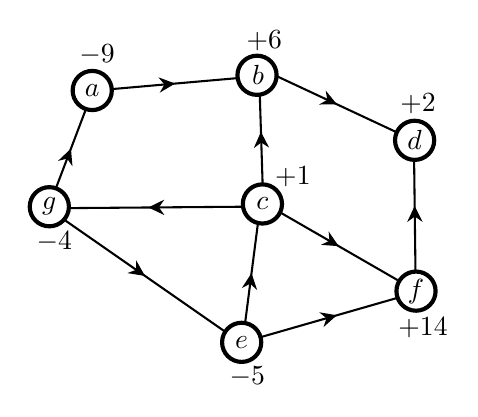
\begin{tikzpicture}[x=0.5pt,y=0.5pt,yscale=-1,xscale=1]
%uncomment if require: \path (0,271); %set diagram left start at 0, and has height of 271

%Straight Lines [id:da5212458340621946] 
\draw [color={rgb, 255:red, 0; green, 0; blue, 0 }  ,draw opacity=1 ][line width=0.75]    (72.5,45) -- (164,37) ;
\draw [shift={(118.25,41)}, rotate = 175] [fill={rgb, 255:red, 0; green, 0; blue, 0 }  ,fill opacity=1 ][line width=0.08]  [draw opacity=0] (11.61,-5.58) -- (0,0) -- (11.61,5.58) -- (7.71,0) -- cycle    ;
%Straight Lines [id:da5107871061349898] 
\draw [color={rgb, 255:red, 0; green, 0; blue, 0 }  ,draw opacity=1 ][line width=0.75]    (278,76) -- (192.5,36) ;
\draw [shift={(235.25,56)}, rotate = 205.07] [fill={rgb, 255:red, 0; green, 0; blue, 0 }  ,fill opacity=1 ][line width=0.08]  [draw opacity=0] (11.61,-5.58) -- (0,0) -- (11.61,5.58) -- (7.71,0) -- cycle    ;
%Straight Lines [id:da33373699050559813] 
\draw [color={rgb, 255:red, 0; green, 0; blue, 0 }  ,draw opacity=1 ][line width=0.75]    (291,96) -- (292,177) ;
\draw [shift={(291.41,129.4)}, rotate = 89.29] [fill={rgb, 255:red, 0; green, 0; blue, 0 }  ,fill opacity=1 ][line width=0.08]  [draw opacity=0] (11.61,-5.58) -- (0,0) -- (11.61,5.58) -- (7.71,0) -- cycle    ;
%Straight Lines [id:da41415742704032066] 
\draw [color={rgb, 255:red, 0; green, 0; blue, 0 }  ,draw opacity=1 ][line width=0.75]    (181,224) -- (278.5,196) ;
\draw [shift={(235.13,208.45)}, rotate = 163.98] [fill={rgb, 255:red, 0; green, 0; blue, 0 }  ,fill opacity=1 ][line width=0.08]  [draw opacity=0] (11.61,-5.58) -- (0,0) -- (11.61,5.58) -- (7.71,0) -- cycle    ;
%Straight Lines [id:da5297018905877636] 
\draw [color={rgb, 255:red, 0; green, 0; blue, 0 }  ,draw opacity=1 ][line width=0.75]    (181.5,113) -- (179.5,50) ;
\draw [shift={(180.32,75.9)}, rotate = 88.18] [fill={rgb, 255:red, 0; green, 0; blue, 0 }  ,fill opacity=1 ][line width=0.08]  [draw opacity=0] (11.61,-5.58) -- (0,0) -- (11.61,5.58) -- (7.71,0) -- cycle    ;
%Straight Lines [id:da9441285731905983] 
\draw [color={rgb, 255:red, 0; green, 0; blue, 0 }  ,draw opacity=1 ][line width=0.75]    (54,59) -- (32,117) ;
\draw [shift={(43,88)}, rotate = 110.77] [fill={rgb, 255:red, 0; green, 0; blue, 0 }  ,fill opacity=1 ][line width=0.08]  [draw opacity=0] (11.61,-5.58) -- (0,0) -- (11.61,5.58) -- (7.71,0) -- cycle    ;
%Straight Lines [id:da3078405450216426] 
\draw [color={rgb, 255:red, 0; green, 0; blue, 0 }  ,draw opacity=1 ][line width=0.75]    (167,130) -- (42,131) ;
\draw [shift={(98.9,130.54)}, rotate = 359.54] [fill={rgb, 255:red, 0; green, 0; blue, 0 }  ,fill opacity=1 ][line width=0.08]  [draw opacity=0] (11.61,-5.58) -- (0,0) -- (11.61,5.58) -- (7.71,0) -- cycle    ;
%Straight Lines [id:da3541622648157198] 
\draw [color={rgb, 255:red, 0; green, 0; blue, 0 }  ,draw opacity=1 ][line width=0.75]    (154,220) -- (39,140) ;
\draw [shift={(96.5,180)}, rotate = 214.82] [fill={rgb, 255:red, 0; green, 0; blue, 0 }  ,fill opacity=1 ][line width=0.08]  [draw opacity=0] (11.61,-5.58) -- (0,0) -- (11.61,5.58) -- (7.71,0) -- cycle    ;
%Straight Lines [id:da720688848918495] 
\draw [color={rgb, 255:red, 0; green, 0; blue, 0 }  ,draw opacity=1 ][line width=0.75]    (279,183) -- (194,134) ;
\draw [shift={(236.5,158.5)}, rotate = 209.96] [fill={rgb, 255:red, 0; green, 0; blue, 0 }  ,fill opacity=1 ][line width=0.08]  [draw opacity=0] (11.61,-5.58) -- (0,0) -- (11.61,5.58) -- (7.71,0) -- cycle    ;
%Straight Lines [id:da4466024070919401] 
\draw [color={rgb, 255:red, 0; green, 0; blue, 0 }  ,draw opacity=1 ][line width=0.75]    (178,143) -- (169,213) ;
\draw [shift={(173.5,178)}, rotate = 97.33] [fill={rgb, 255:red, 0; green, 0; blue, 0 }  ,fill opacity=1 ][line width=0.08]  [draw opacity=0] (11.61,-5.58) -- (0,0) -- (11.61,5.58) -- (7.71,0) -- cycle    ;

% Text Node
\draw (47.24,11.06) node [anchor=north west][inner sep=0.75pt]   [align=left] {$\displaystyle -9$};
% Text Node
\draw  [line width=1.5]   (27.38, 130) circle [x radius= 14.15, y radius= 14.15]   ;
\draw (27.38,130) node   [align=left] {$\displaystyle g$};
% Text Node
\draw  [line width=1.5]   (58.38, 46) circle [x radius= 14.15, y radius= 14.15]   ;
\draw (58.38,46) node   [align=left] {$\displaystyle a$};
% Text Node
\draw  [line width=1.5]   (177.48, 35) circle [x radius= 14.15, y radius= 14.15]   ;
\draw (171.98,35) node [anchor=west] [inner sep=0.75pt]   [align=left] {$\displaystyle b$};
% Text Node
\draw  [line width=1.5]   (181.38, 128) circle [x radius= 14.15, y radius= 14.15]   ;
\draw (181.38,128) node   [align=left] {$\displaystyle c$};
% Text Node
\draw  [line width=1.5]   (291.38, 82) circle [x radius= 14.15, y radius= 14.15]   ;
\draw (291.38,82) node   [align=left] {$\displaystyle d$};
% Text Node
\draw  [line width=1.5]   (166.38, 228) circle [x radius= 14.15, y radius= 14.15]   ;
\draw (166.38,228) node   [align=left] {$\displaystyle e$};
% Text Node
\draw  [line width=1.5]   (292.38, 191) circle [x radius= 14.15, y radius= 14.15]   ;
\draw (292.38,191) node   [align=left] {$\displaystyle f$};
% Text Node
\draw (16.24,146.06) node [anchor=north west][inner sep=0.75pt]   [align=left] {$\displaystyle -4$};
% Text Node
\draw (279.24,46.06) node [anchor=north west][inner sep=0.75pt]   [align=left] {$\displaystyle +2$};
% Text Node
\draw (155.75,244) node [anchor=north west][inner sep=0.75pt]   [align=left] {$\displaystyle -5$};
% Text Node
\draw (168,1) node [anchor=north west][inner sep=0.75pt]   [align=left] {$\displaystyle +6$};
% Text Node
\draw (277.75,208) node [anchor=north west][inner sep=0.75pt]   [align=left] {$\displaystyle +14$};
% Text Node
\draw (188.75,99) node [anchor=north west][inner sep=0.75pt]   [align=left] {$\displaystyle +1$};


\end{tikzpicture}

}
\caption{An example of project selection problem. $\{g,c,e\}$ satisfies the
prerequisite condition; $\{b,c,d\}$ does not satisfies the prerequisite condition.
The optimal solution for this example is $V_1 = \{g,c,e,f\}$, as $V_1$ satisfies the prerequisite condition
and that its total profit $\sum_{v\in V_1} p(v) = 6$ is maximized.}
\label{fig:ps1}
\end{figure}

The project selection problem is an abstracted formulation that well models
application scenarios that involves making decisions over a set of things that depend on each other.
For instance, this formulation can be used to model the election of courses. Specifically, each vertex
represents a course and the prerequisites are modeled as edges. Each course is associated with an estimated
gain/loss on the overall GPA. Hence, this formulation seeks a subset of courses~(satisfying the prerequisite condition, of course)
so as to maximize the net gain over one's GPA. Another application scanario is
running a company, where one needs to decide over a set of ``items'' such as
hiring people, purchasing equipments, making products, etc. These items clearly depend on each other.
For examples, making a product requires hiring people with certain expertise and purchasing certain equipments;
a certain equipment can be used by several products, etc. The items can be modeled as vertices and their dependencies
be modeled as edges. Items may have an estimated cost~(negative profit) or gain~(positive profit). Deciding on the items so as to
maximize the total profit is clearly another instance of the project selection problem.

We design algorithm to solve this problem. The brute-force approach
enumerates all possible subsets~(which projects to select), and for each subset
one can examine if it satisfies the prerequisite condition, and if it does, calculate
its total profit and keep track of the one with maximized total profit. 
Since there are $2^{|V|}$ possible subsets, this brute-force algorithm certainly runs in exponential time.

We now design a polynomial-time algorithm for above problem, by
reducing/transforming it into a network flow problem.
Recall that, such reduction involves a 3-step procedure. First,
constructing a network $(G', s, t, c)$ based on the input graph $G$ and profit
$p(\cdot)$; second, using an existing algorithm for max-flow to obtain the
maximum-flow $f^*$ and/or minimum $s$-$t$ cut $(S^*, T^*)$ of the network $G'$;
third, find the optimal solution $V_1$, using the found $f^*$ and/or $(S^*, T^*)$.

You may pause now to think about how we apply this framework to solve the maximum-matching problem for bipartite graph.
For that problem, we establish that, there exists a one-to-one correspondence between any matching $M$ of the bipartite
graph and any (integral) flow $f$ of the constructed network, and that $|M| = |f|$. Hence, finding maximum-matching of the
bipartite graph is equivalent to finding maximum-flow of the network. 
But it is hard to find any connection between the project selection problem with flow. In fact, here we essentially seek
a partition of vertices---projects we select and projects we do not select, which is exactly a cut!
Hence, for the project selection problem, we instead will establish a
one-to-one correspondence between any selection and any $s$-$t$ cut
of the constructed network, and we will also show that minimizing the
total profit of the selected projects
is equivalent to finding the minimum $s$-$t$ cut of the network.

We now work out the details of above roadmap. In step \#1, we construct the network $(G' = (V',E'),s,t,c)$ as follows.
See Figure~\ref{fig:ps2}. The directed graph $G'$ incorporates the given graph $G = (V, E)$, not a surprise.
We add a source $s$ and a sink $t$, i.e., $V' = V\cup \{s,t\}$. We connect $s$ to each project with negative profit, and
connect each project with positive profit to sink $t$. Formally, edges in the network is: 
$E' = E\cup \{(s,v)\mid p(v) < 0\} \cup \{(v,t)\mid p(v) > 0\}$.
Now we assign capacities: edges in $E$, i.e., these in the given graph $G$, will have a capacity of $\infty$;
edge $(s,v)$ will have a capacity of $-p(v)$;
edge $(v,t)$ will have a capacity of $p(v)$.
The reasons behind such construction will be revealed when proving the correctness of the algorithm.

\begin{figure}[!h]
\centering{

\tikzset{every picture/.style={line width=0.75pt}} %set default line width to 0.75pt        

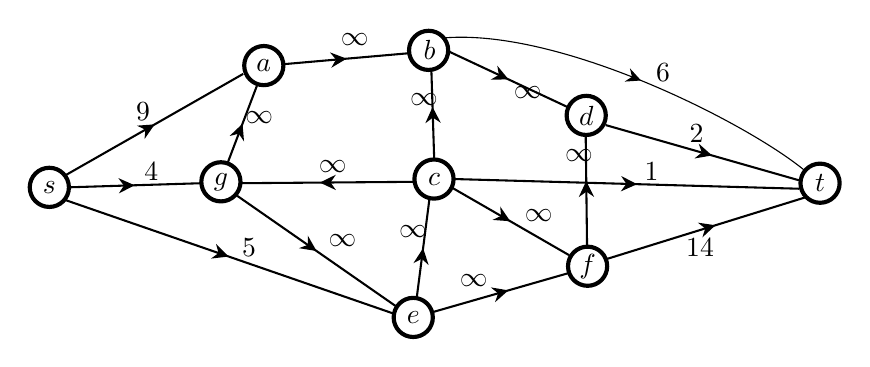
\begin{tikzpicture}[x=0.5pt,y=0.5pt,yscale=-1,xscale=1]
%uncomment if require: \path (0,271); %set diagram left start at 0, and has height of 271

%Straight Lines [id:da5212458340621946] 
\draw [color={rgb, 255:red, 0; green, 0; blue, 0 }  ,draw opacity=1 ][line width=0.75]    (227.5,50) -- (319,42) ;
\draw [shift={(273.25,46)}, rotate = 175] [fill={rgb, 255:red, 0; green, 0; blue, 0 }  ,fill opacity=1 ][line width=0.08]  [draw opacity=0] (11.61,-5.58) -- (0,0) -- (11.61,5.58) -- (7.71,0) -- cycle    ;
%Straight Lines [id:da5107871061349898] 
\draw [color={rgb, 255:red, 0; green, 0; blue, 0 }  ,draw opacity=1 ][line width=0.75]    (433,81) -- (347.5,41) ;
\draw [shift={(390.25,61)}, rotate = 205.07] [fill={rgb, 255:red, 0; green, 0; blue, 0 }  ,fill opacity=1 ][line width=0.08]  [draw opacity=0] (11.61,-5.58) -- (0,0) -- (11.61,5.58) -- (7.71,0) -- cycle    ;
%Straight Lines [id:da33373699050559813] 
\draw [color={rgb, 255:red, 0; green, 0; blue, 0 }  ,draw opacity=1 ][line width=0.75]    (446,101) -- (447,182) ;
\draw [shift={(446.41,134.4)}, rotate = 89.29] [fill={rgb, 255:red, 0; green, 0; blue, 0 }  ,fill opacity=1 ][line width=0.08]  [draw opacity=0] (11.61,-5.58) -- (0,0) -- (11.61,5.58) -- (7.71,0) -- cycle    ;
%Straight Lines [id:da41415742704032066] 
\draw [color={rgb, 255:red, 0; green, 0; blue, 0 }  ,draw opacity=1 ][line width=0.75]    (336,229) -- (433.5,201) ;
\draw [shift={(390.13,213.45)}, rotate = 163.98] [fill={rgb, 255:red, 0; green, 0; blue, 0 }  ,fill opacity=1 ][line width=0.08]  [draw opacity=0] (11.61,-5.58) -- (0,0) -- (11.61,5.58) -- (7.71,0) -- cycle    ;
%Straight Lines [id:da5297018905877636] 
\draw [color={rgb, 255:red, 0; green, 0; blue, 0 }  ,draw opacity=1 ][line width=0.75]    (336.5,118) -- (334.5,55) ;
\draw [shift={(335.32,80.9)}, rotate = 88.18] [fill={rgb, 255:red, 0; green, 0; blue, 0 }  ,fill opacity=1 ][line width=0.08]  [draw opacity=0] (11.61,-5.58) -- (0,0) -- (11.61,5.58) -- (7.71,0) -- cycle    ;
%Straight Lines [id:da9441285731905983] 
\draw [color={rgb, 255:red, 0; green, 0; blue, 0 }  ,draw opacity=1 ][line width=0.75]    (209,64) -- (187,122) ;
\draw [shift={(198,93)}, rotate = 110.77] [fill={rgb, 255:red, 0; green, 0; blue, 0 }  ,fill opacity=1 ][line width=0.08]  [draw opacity=0] (11.61,-5.58) -- (0,0) -- (11.61,5.58) -- (7.71,0) -- cycle    ;
%Straight Lines [id:da3078405450216426] 
\draw [color={rgb, 255:red, 0; green, 0; blue, 0 }  ,draw opacity=1 ][line width=0.75]    (322,135) -- (197,136) ;
\draw [shift={(253.9,135.54)}, rotate = 359.54] [fill={rgb, 255:red, 0; green, 0; blue, 0 }  ,fill opacity=1 ][line width=0.08]  [draw opacity=0] (11.61,-5.58) -- (0,0) -- (11.61,5.58) -- (7.71,0) -- cycle    ;
%Straight Lines [id:da3541622648157198] 
\draw [color={rgb, 255:red, 0; green, 0; blue, 0 }  ,draw opacity=1 ][line width=0.75]    (309,225) -- (194,145) ;
\draw [shift={(251.5,185)}, rotate = 214.82] [fill={rgb, 255:red, 0; green, 0; blue, 0 }  ,fill opacity=1 ][line width=0.08]  [draw opacity=0] (11.61,-5.58) -- (0,0) -- (11.61,5.58) -- (7.71,0) -- cycle    ;
%Straight Lines [id:da720688848918495] 
\draw [color={rgb, 255:red, 0; green, 0; blue, 0 }  ,draw opacity=1 ][line width=0.75]    (434,188) -- (349,139) ;
\draw [shift={(391.5,163.5)}, rotate = 209.96] [fill={rgb, 255:red, 0; green, 0; blue, 0 }  ,fill opacity=1 ][line width=0.08]  [draw opacity=0] (11.61,-5.58) -- (0,0) -- (11.61,5.58) -- (7.71,0) -- cycle    ;
%Straight Lines [id:da4466024070919401] 
\draw [color={rgb, 255:red, 0; green, 0; blue, 0 }  ,draw opacity=1 ][line width=0.75]    (333,148) -- (324,218) ;
\draw [shift={(328.5,183)}, rotate = 97.33] [fill={rgb, 255:red, 0; green, 0; blue, 0 }  ,fill opacity=1 ][line width=0.08]  [draw opacity=0] (11.61,-5.58) -- (0,0) -- (11.61,5.58) -- (7.71,0) -- cycle    ;
%Straight Lines [id:da19156407920574714] 
\draw [color={rgb, 255:red, 0; green, 0; blue, 0 }  ,draw opacity=1 ][line width=0.75]    (198.5,57) -- (70.5,130) ;
\draw [shift={(134.5,93.5)}, rotate = 150.3] [fill={rgb, 255:red, 0; green, 0; blue, 0 }  ,fill opacity=1 ][line width=0.08]  [draw opacity=0] (11.61,-5.58) -- (0,0) -- (11.61,5.58) -- (7.71,0) -- cycle    ;
%Straight Lines [id:da6856541088604527] 
\draw [color={rgb, 255:red, 0; green, 0; blue, 0 }  ,draw opacity=1 ][line width=0.75]    (168.5,136) -- (71.5,139) ;
\draw [shift={(120,137.5)}, rotate = 178.23] [fill={rgb, 255:red, 0; green, 0; blue, 0 }  ,fill opacity=1 ][line width=0.08]  [draw opacity=0] (11.61,-5.58) -- (0,0) -- (11.61,5.58) -- (7.71,0) -- cycle    ;
%Straight Lines [id:da6199102597257959] 
\draw [color={rgb, 255:red, 0; green, 0; blue, 0 }  ,draw opacity=1 ][line width=0.75]    (306.5,230) -- (69.5,148) ;
\draw [shift={(188,189)}, rotate = 199.09] [fill={rgb, 255:red, 0; green, 0; blue, 0 }  ,fill opacity=1 ][line width=0.08]  [draw opacity=0] (11.61,-5.58) -- (0,0) -- (11.61,5.58) -- (7.71,0) -- cycle    ;
%Straight Lines [id:da9810487383568949] 
\draw [color={rgb, 255:red, 0; green, 0; blue, 0 }  ,draw opacity=1 ][line width=0.75]    (600.5,134) -- (460.5,94) ;
\draw [shift={(537.33,115.95)}, rotate = 195.95] [fill={rgb, 255:red, 0; green, 0; blue, 0 }  ,fill opacity=1 ][line width=0.08]  [draw opacity=0] (11.61,-5.58) -- (0,0) -- (11.61,5.58) -- (7.71,0) -- cycle    ;
%Curve Lines [id:da06719487778357702] 
\draw    (343.5,31) .. controls (428.5,24) and (563.5,93) .. (604.5,127) ;
\draw [shift={(486.03,61.78)}, rotate = 201.88] [fill={rgb, 255:red, 0; green, 0; blue, 0 }  ][line width=0.08]  [draw opacity=0] (10.72,-5.15) -- (0,0) -- (10.72,5.15) -- (7.12,0) -- cycle    ;
%Straight Lines [id:da5887320294982179] 
\draw [color={rgb, 255:red, 0; green, 0; blue, 0 }  ,draw opacity=1 ][line width=0.75]    (605.5,146) -- (460.5,191) ;
\draw [shift={(539.78,166.4)}, rotate = 162.76] [fill={rgb, 255:red, 0; green, 0; blue, 0 }  ,fill opacity=1 ][line width=0.08]  [draw opacity=0] (11.61,-5.58) -- (0,0) -- (11.61,5.58) -- (7.71,0) -- cycle    ;
%Straight Lines [id:da573517504295797] 
\draw [color={rgb, 255:red, 0; green, 0; blue, 0 }  ,draw opacity=1 ][line width=0.75]    (600.5,140) -- (351.5,133) ;
\draw [shift={(483.1,136.7)}, rotate = 181.61] [fill={rgb, 255:red, 0; green, 0; blue, 0 }  ,fill opacity=1 ][line width=0.08]  [draw opacity=0] (11.61,-5.58) -- (0,0) -- (11.61,5.58) -- (7.71,0) -- cycle    ;

% Text Node
\draw (119.24,76.06) node [anchor=north west][inner sep=0.75pt]   [align=left] {$\displaystyle 9$};
% Text Node
\draw  [line width=1.5]   (182.38, 135) circle [x radius= 14.15, y radius= 14.15]   ;
\draw (182.38,135) node   [align=left] {$\displaystyle g$};
% Text Node
\draw  [line width=1.5]   (213.38, 51) circle [x radius= 14.15, y radius= 14.15]   ;
\draw (213.38,51) node   [align=left] {$\displaystyle a$};
% Text Node
\draw  [line width=1.5]   (332.48, 40) circle [x radius= 14.15, y radius= 14.15]   ;
\draw (326.98,40) node [anchor=west] [inner sep=0.75pt]   [align=left] {$\displaystyle b$};
% Text Node
\draw  [line width=1.5]   (336.38, 133) circle [x radius= 14.15, y radius= 14.15]   ;
\draw (336.38,133) node   [align=left] {$\displaystyle c$};
% Text Node
\draw  [line width=1.5]   (446.38, 87) circle [x radius= 14.15, y radius= 14.15]   ;
\draw (446.38,87) node   [align=left] {$\displaystyle d$};
% Text Node
\draw  [line width=1.5]   (321.38, 233) circle [x radius= 14.15, y radius= 14.15]   ;
\draw (321.38,233) node   [align=left] {$\displaystyle e$};
% Text Node
\draw  [line width=1.5]   (447.38, 196) circle [x radius= 14.15, y radius= 14.15]   ;
\draw (447.38,196) node   [align=left] {$\displaystyle f$};
% Text Node
\draw (125.24,119.06) node [anchor=north west][inner sep=0.75pt]   [align=left] {$\displaystyle 4$};
% Text Node
\draw (519.24,92.06) node [anchor=north west][inner sep=0.75pt]   [align=left] {$\displaystyle 2$};
% Text Node
\draw (195.75,174) node [anchor=north west][inner sep=0.75pt]   [align=left] {$\displaystyle 5$};
% Text Node
\draw (495,48) node [anchor=north west][inner sep=0.75pt]   [align=left] {$\displaystyle 6$};
% Text Node
\draw (516.75,174) node [anchor=north west][inner sep=0.75pt]   [align=left] {$\displaystyle 14$};
% Text Node
\draw (486.75,119) node [anchor=north west][inner sep=0.75pt]   [align=left] {$\displaystyle 1$};
% Text Node
\draw  [line width=1.5]   (58.38, 139) circle [x radius= 14.15, y radius= 14.15]   ;
\draw (58.38,139) node   [align=left] {$\displaystyle s$};
% Text Node
\draw  [line width=1.5]   (615.38, 136) circle [x radius= 14.15, y radius= 14.15]   ;
\draw (615.38,136) node   [align=left] {$\displaystyle t$};
% Text Node
\draw (267.24,26.06) node [anchor=north west][inner sep=0.75pt]   [align=left] {$\displaystyle \infty $};
% Text Node
\draw (198.24,82.06) node [anchor=north west][inner sep=0.75pt]   [align=left] {$\displaystyle \infty $};
% Text Node
\draw (251.24,118.06) node [anchor=north west][inner sep=0.75pt]   [align=left] {$\displaystyle \infty $};
% Text Node
\draw (258.24,171.06) node [anchor=north west][inner sep=0.75pt]   [align=left] {$\displaystyle \infty $};
% Text Node
\draw (309.24,165.06) node [anchor=north west][inner sep=0.75pt]   [align=left] {$\displaystyle \infty $};
% Text Node
\draw (353.24,200.06) node [anchor=north west][inner sep=0.75pt]   [align=left] {$\displaystyle \infty $};
% Text Node
\draw (400.24,153.06) node [anchor=north west][inner sep=0.75pt]   [align=left] {$\displaystyle \infty $};
% Text Node
\draw (429.24,110.06) node [anchor=north west][inner sep=0.75pt]   [align=left] {$\displaystyle \infty $};
% Text Node
\draw (317.24,69.06) node [anchor=north west][inner sep=0.75pt]   [align=left] {$\displaystyle \infty $};
% Text Node
\draw (392.25,64) node [anchor=north west][inner sep=0.75pt]   [align=left] {$\displaystyle \infty $};


\end{tikzpicture}

}
\caption{The constructed network $(G',s,t,c)$ for the example in Figure~\ref{fig:ps1}.}
\label{fig:ps2}
\end{figure}

In step \#2, we find a minimum $s$-$t$ cut $(S^*, T^*)$ of above network $(G',s,t,c)$.
In step \#3, the algorithm simply returns projects in $t$-side, i.e., returning $V_1^* = T^*\setminus \{t\}$.
See Figure~\ref{fig:ps3}.

\begin{figure}[!h]
\centering{\input{ps3}}
\caption{The minimum $s$-$t$ cut $(S^*, T^*)$ of the network $G'$ in Figure~\ref{fig:ps2}.
Therefore, for this example, the algorithm returns $V_1^* = T^*\setminus\{t\} = \{g,c,e,f\}$.}
\label{fig:ps3}
\end{figure}

We now prove that the above algorithm is correct, i.e., to prove that the returned $V_1^*$ satisfies
the prerequisite condition and that $\sum_{v\in V_1^*} p(v)$ is maximized.
To achieve this, we establish the one-to-one correspondence between 
selections and $s$-$t$ cuts of the built network.
Formally, let $V_1 \subset V$ be an arbitrary selection~(i.e., a subset of projects). 
Let $T = V_1\cup \{t\}$ and $S = (V\setminus V_1)\cup \{s\}$.  
Clearly, $(S,T)$ forms an $s$-$t$ cut of the network.  
%\begin{fact}
%The returned $V_1^* = T^*\setminus\{t\}$ satisfies the prerequisite condition.
%\end{fact}

\begin{fact}
%Let $V_1 \subset V$ be an arbitrary subset of $V$. Let $T = V_1\cup \{t\}$ and
%let $S = (V\setminus V_1)\cup \{s\}$.  Clearly, $(S,T)$ forms an $s$-$t$ cut of 
%the network.  
$V_1$ satisfies the prerequisite condition if and only if $c(S, T) < \infty$.
\label{fact1}
\end{fact}

You may check a couple of examples to fully understand above statement.
See Figure~\ref{fig:ps4}. 
%In above example, $V_1$ satisfies the prerequisite
%condition, because, by definition, there is no such edge $(u, v)$ where $v\in V_1$ but $u\not\in V_1$.
%Hence, the none of edges in $E$, which have capacity of $\infty$, belongs to the cut-edges.
%In the example below, $V_1$ does not satisfy the prerequisite
%condition, because, there exists edge $(u, v)$ where $v\in V_1$ and $u\not\in V_1$, for example edge $(a,b)$.
%This edge is therefore one of the cut-edges of cut $(S,T)$. Since the capacity of this edge is $\infty$,
%the capacity of $(S,T)$ must be also $\infty$.

\begin{figure}[!h]
\centering{\input{ps4}}
\caption{Above: $V_1 = \{g,c,e\}$ which satisfies the prerequisite condition;
the corresponding cut capacity $c(S, T) = 31 < \infty$.
Below: $V_1 = \{b,c,d\}$ which does not satisfy the prerequisite condition;
the corresponding cut capacity $c(S, T) = \infty$.
	In both examples, cut-edges are marked in blue.  }
\label{fig:ps4}
\end{figure}


\emph{Proof of Fact~\ref{fact1}.} 
If $V_1$ satisfies the prerequisite
condition~(see the top example of Figure~\ref{fig:ps4}), then, by definition, there is no such edge $(u, v)$ where $v\in V_1$ but $u\not\in V_1$.
Hence, none of edges in $E$, which have capacity of $\infty$, belongs to the cut-edges of cut $(S,T)$.  So we must have $c(S,T) < \infty$.
If $V_1$ does not satisfy the prerequisite
condition~(see the bottom example in Figure~\ref{fig:ps4}), 
then there exists edge $(u, v)$ where $v\in V_1$ and $u\not\in V_1$.
This edge is therefore one of the cut-edges of cut $(S,T)$. 
Also because the capacity of this edge is $\infty$,
we must have $c(S,T) = \infty$.  \qed
%Let $E(S,T)$ be the cut-edges of cut $(S, T)$. Note that in the network, only edges in $E$~(i.e., edges
%in the given directed graph, rather than these connecting to $s$ or $t$) are assigned 
%a capacity of $\infty$. Hence, $c(S, T) < \infty$ is equivalent to $E(S,T) \cap E=\emptyset$.
%If $V_1$ satisfies the prerequisite condition, then by definition, it means for each $v\in V_1$ and $(u,v)\in E$
%then $u\in V_1$. Hence, none of the edges in $E$ is an cut-edge, i.e., $E(S,T) \cap E=\emptyset$.
%For the other side, 

%Assume conversely that $V_1^*$ does not satisfy the prerequisite condition.
%This means that there exists edge $(u,v)\in E$ such that $v\in V_1^*$ but $u\not\in V_1^*$.
%Since $V_1^* = T^*\setminus\{t\}$, this implies that $v\in T^*$ and $u\in S^*$.
%Hence, $(u,v)$ is one cut-edge of cut $(S^*, T^*)$. According to the construction
%of network $G'$, since $(u,v)\in E$, its capacity $c(u,v) = \infty$.
%This consequently implies $c(S^*, T^*) = \infty$. This is a contradiction
%to the fact that $(S^*, T^*)$ is a minimum $s$-$t$ cut, as we know that 

In the network $G'$, $s$-$t$ cut $(S,T)$ with $c(S, T) < \infty$ exists; for example the $s$-$t$ cut with just $\{s\}$ on one side.
Hence, the minimum $s$-$t$ cut $(S^*, T^*)$ of the network must have that $c(S^*, T^*) < \infty$, since it is minimum.
Combining with above Fact~\ref{fact1}, we have the following: %The proves the follat, $V_1^* = T^*\setminus\{t\}$ must satisfy the prerequisite condition:
\begin{fact}
The returned $V_1^* = T^*\setminus\{t\}$ satisfies the prerequisite condition.
\end{fact}

It should be clear now why we assign infinite capacity to edges in $E$ when constructing the network $G'$.
This is simply because doing so guarantees that the returned projects satisfies the prerequisite condition.
In other words, assigning these edges an infinite capacity \emph{avoids} the cut-edges go through any of them,
ensuring that the projects on the $t$-side satisfies the prerequisite condition.


We now prove that $V_1^*$ maximizes the total profit, by establishing the quantitative relationship between the
total profit of any selection and the capacity of the corresponding $s$-$t$ cut.
Let $V_1 \subset V$ be a subset of $V$ that satisfies the prerequisite condition. 
Let $(S,T)$ be the corresponding $s$-$t$ cut, where $T = V_1\cup \{t\}$ and
let $S = (V\setminus V_1)\cup \{s\}$.  %We know that $c(S, T) < \infty$.
$S$ and $T$ partition all projects~(vertices in $V$) into two classes.
Combining whether a project has a negative or positive profit, 
all projects are now partitioned into four categories: $S_+$, $S_-$, $T_+$, and $T_-$, where
$S_+$ consists of projects in $S$ while having positive profit~(similar for other three categories).
Now the network $G'$ can be sketched in Figure~\ref{fig:ps5}.
Note that $s$ connects to projects with negative profit, i.e., $S_-\cup T_-$,
and $t$ is connected from projects with positive profit, i.e., $S_+\cup T_+$.
Also note that there is no edge from $S_-\cup S_+$ to $T_-\cup T_+$ because we assume that $V_1$, which is $T_-\cup T_+$, 
satisfies the prerequisite condition~(see Fact~\ref{fact1}). 

\begin{figure}[!h]
\centering{

\tikzset{every picture/.style={line width=0.75pt}} %set default line width to 0.75pt        

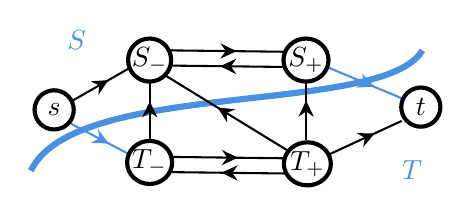
\begin{tikzpicture}[x=0.5pt,y=0.5pt,yscale=-1,xscale=1]
%uncomment if require: \path (0,219); %set diagram left start at 0, and has height of 219

%Curve Lines [id:da293114086641606] 
\draw [color={rgb, 255:red, 74; green, 144; blue, 226 }  ,draw opacity=1 ][line width=2.25]    (44.5,171) .. controls (76.5,104) and (299.5,132) .. (327.5,84) ;
%Straight Lines [id:da07818022990875795] 
\draw [color={rgb, 255:red, 0; green, 0; blue, 0 }  ,draw opacity=1 ][line width=0.75]    (115.5,97) -- (73.5,121) ;
\draw [shift={(100.66,105.48)}, rotate = 150.26] [fill={rgb, 255:red, 0; green, 0; blue, 0 }  ,fill opacity=1 ][line width=0.08]  [draw opacity=0] (11.61,-5.58) -- (0,0) -- (11.61,5.58) -- (7.71,0) -- cycle    ;
%Straight Lines [id:da13447323458917793] 
\draw [color={rgb, 255:red, 74; green, 144; blue, 226 }  ,draw opacity=1 ][line width=0.75]    (115.5,159) -- (73.5,137) ;
\draw [shift={(100.79,151.29)}, rotate = 207.65] [fill={rgb, 255:red, 74; green, 144; blue, 226 }  ,fill opacity=1 ][line width=0.08]  [draw opacity=0] (11.61,-5.58) -- (0,0) -- (11.61,5.58) -- (7.71,0) -- cycle    ;
%Straight Lines [id:da8494415517252689] 
\draw [color={rgb, 255:red, 74; green, 144; blue, 226 }  ,draw opacity=1 ][line width=0.75]    (313.5,119) -- (258.5,96) ;
\draw [shift={(292.55,110.24)}, rotate = 202.69] [fill={rgb, 255:red, 74; green, 144; blue, 226 }  ,fill opacity=1 ][line width=0.08]  [draw opacity=0] (11.61,-5.58) -- (0,0) -- (11.61,5.58) -- (7.71,0) -- cycle    ;
%Straight Lines [id:da07398074829543488] 
\draw [color={rgb, 255:red, 0; green, 0; blue, 0 }  ,draw opacity=1 ][line width=0.75]    (312.5,135) -- (260.5,159) ;
\draw [shift={(292.95,144.02)}, rotate = 155.22] [fill={rgb, 255:red, 0; green, 0; blue, 0 }  ,fill opacity=1 ][line width=0.08]  [draw opacity=0] (11.61,-5.58) -- (0,0) -- (11.61,5.58) -- (7.71,0) -- cycle    ;
%Straight Lines [id:da19965646081311195] 
\draw [color={rgb, 255:red, 0; green, 0; blue, 0 }  ,draw opacity=1 ][line width=0.75]    (227.5,85) -- (144.5,84) ;
\draw [shift={(193.1,84.59)}, rotate = 180.69] [fill={rgb, 255:red, 0; green, 0; blue, 0 }  ,fill opacity=1 ][line width=0.08]  [draw opacity=0] (11.61,-5.58) -- (0,0) -- (11.61,5.58) -- (7.71,0) -- cycle    ;
%Straight Lines [id:da5020627943874022] 
\draw [color={rgb, 255:red, 0; green, 0; blue, 0 }  ,draw opacity=1 ][line width=0.75]    (228.5,96) -- (145.5,95) ;
\draw [shift={(181.4,95.43)}, rotate = 0.69] [fill={rgb, 255:red, 0; green, 0; blue, 0 }  ,fill opacity=1 ][line width=0.08]  [draw opacity=0] (11.61,-5.58) -- (0,0) -- (11.61,5.58) -- (7.71,0) -- cycle    ;
%Straight Lines [id:da3615258313224192] 
\draw [color={rgb, 255:red, 0; green, 0; blue, 0 }  ,draw opacity=1 ][line width=0.75]    (228.5,162) -- (145.5,161) ;
\draw [shift={(194.1,161.59)}, rotate = 180.69] [fill={rgb, 255:red, 0; green, 0; blue, 0 }  ,fill opacity=1 ][line width=0.08]  [draw opacity=0] (11.61,-5.58) -- (0,0) -- (11.61,5.58) -- (7.71,0) -- cycle    ;
%Straight Lines [id:da9852604392093721] 
\draw [color={rgb, 255:red, 0; green, 0; blue, 0 }  ,draw opacity=1 ][line width=0.75]    (229.5,173) -- (146.5,172) ;
\draw [shift={(182.4,172.43)}, rotate = 0.69] [fill={rgb, 255:red, 0; green, 0; blue, 0 }  ,fill opacity=1 ][line width=0.08]  [draw opacity=0] (11.61,-5.58) -- (0,0) -- (11.61,5.58) -- (7.71,0) -- cycle    ;
%Straight Lines [id:da8921257697911721] 
\draw [color={rgb, 255:red, 0; green, 0; blue, 0 }  ,draw opacity=1 ][line width=0.75]    (130.5,107) -- (130.5,149) ;
\draw [shift={(130.5,120.9)}, rotate = 90] [fill={rgb, 255:red, 0; green, 0; blue, 0 }  ,fill opacity=1 ][line width=0.08]  [draw opacity=0] (11.61,-5.58) -- (0,0) -- (11.61,5.58) -- (7.71,0) -- cycle    ;
%Straight Lines [id:da2647924953727303] 
\draw [color={rgb, 255:red, 0; green, 0; blue, 0 }  ,draw opacity=1 ][line width=0.75]    (243.5,106) -- (243.5,149) ;
\draw [shift={(243.5,120.4)}, rotate = 90] [fill={rgb, 255:red, 0; green, 0; blue, 0 }  ,fill opacity=1 ][line width=0.08]  [draw opacity=0] (11.61,-5.58) -- (0,0) -- (11.61,5.58) -- (7.71,0) -- cycle    ;
%Straight Lines [id:da598001554052235] 
\draw [color={rgb, 255:red, 0; green, 0; blue, 0 }  ,draw opacity=1 ][line width=0.75]    (141.5,102) -- (229.5,156) ;
\draw [shift={(179.45,125.29)}, rotate = 31.53] [fill={rgb, 255:red, 0; green, 0; blue, 0 }  ,fill opacity=1 ][line width=0.08]  [draw opacity=0] (11.61,-5.58) -- (0,0) -- (11.61,5.58) -- (7.71,0) -- cycle    ;

% Text Node
\draw  [line width=1.5]   (130.38, 91) circle [x radius= 15.56, y radius= 15.56]   ;
\draw (130.38,91) node   [align=left] {$\displaystyle S_{-}$};
% Text Node
\draw  [line width=1.5]   (130.38, 165) circle [x radius= 16.26, y radius= 15.56]   ;
\draw (130.38,165) node   [align=left] {$\displaystyle T_{-}$};
% Text Node
\draw  [line width=1.5]   (243.38, 91) circle [x radius= 16.26, y radius= 15.56]   ;
\draw (243.38,91) node   [align=left] {$\displaystyle S_{+}$};
% Text Node
\draw  [line width=1.5]   (244.38, 166) circle [x radius= 16.97, y radius= 15.56]   ;
\draw (244.38,166) node   [align=left] {$\displaystyle T_{+}$};
% Text Node
\draw  [line width=1.5]   (61.38, 127) circle [x radius= 14.15, y radius= 14.15]   ;
\draw (61.38,127) node   [align=left] {$\displaystyle s$};
% Text Node
\draw  [line width=1.5]   (326.38, 125) circle [x radius= 14.15, y radius= 14.15]   ;
\draw (326.38,125) node   [align=left] {$\displaystyle t$};
% Text Node
\draw (69,68) node [anchor=north west][inner sep=0.75pt]  [color={rgb, 255:red, 74; green, 144; blue, 226 }  ,opacity=1 ] [align=left] {$\displaystyle S$};
% Text Node
\draw (311,162) node [anchor=north west][inner sep=0.75pt]  [color={rgb, 255:red, 74; green, 144; blue, 226 }  ,opacity=1 ] [align=left] {$\displaystyle T$};


\end{tikzpicture}

}
\caption{Sketch of the network $G'$ for an $s$-$t$ cut $(S,T)$. }
\label{fig:ps5}
\end{figure}

Now let's establish the connection between capacity of $(S,T)$ and profit of $V_1$.
Note that the cut-edges of $(S,T)$ consists of edges from $s$ to $T_-$ and edges from $S_+$ to $t$.
We have: $c(S, T) = \sum_{v\in T_-} -p(v) + \sum_{v\in S_+} p(v)$.
The total profit of $V_1$ is: $\sum_{v\in V_1} p(v) = \sum_{v\in T_-} p(v) + \sum_{v\in T_+} p(v)$.
We sum up both sides. Note that term $\sum_{v\in T_-} p(v)$ cancels out.
We have $c(S, T) + \sum_{v\in V_1} p(v) = \sum_{v\in S_+} p(v) + \sum_{v\in T_+} p(v)$.
Note that the right side is exactly the total profit of projects with positive profit, i.e., $\sum_{v\in V: p(v) > 0} p(v)$,
which is independent of the $V_1$ or $(S,T)$. In other words, 
$c(S, T) + \sum_{v\in V_1} p(v)$ is a constant! Hence, minimizing one term is equivalent to maximizing the other. 
Since the algorithm finds $(S^*, T^*)$ which minimizes $c(S,T)$, the resulting $V_1^*$ must
have the maximized total profit. This is summarized below, which also concludes the proof.
\begin{fact}
The returned $V_1^* = T^*\setminus\{t\}$ maximizes the total profit.
\end{fact}

The time complexity of the algorithm~(i.e., the 3 steps) is dominated by the time complexity
of calling a max-flow solver. Note that the Ford-Fulkson algorithm does not run in polynomial-time~(it in facts
runs in pseudo-polynomial-time). But there exists polynomial-time algorithm for maximum-flow, for example
the Push-Relabel algorithm. Hence, the algorithm for project selection problem can be solved in polynomial-time as well.
